\documentclass[12pt, a4paper]{article}
\usepackage[UTF8, zihao=-4]{ctex}
\usepackage{fontspec}
\setmainfont{Times New Roman}
\usepackage[top=1.5cm, bottom=1.5cm, left=1.2cm, right=1.2cm, headheight=15pt, includehead]{geometry}
\usepackage{graphicx}
\usepackage{float}
\usepackage{fancyhdr}
\usepackage{eso-pic}
\usepackage{tikz}
\usepackage{setspace}

% 水印（前景层，覆盖图片）
\AddToShipoutPictureFG{%
  \begin{tikzpicture}[overlay, remember picture]
    \node[at=(current page.center), opacity=0.12, rotate=45,
      font=\sffamily\bfseries\fontsize{48}{48}\selectfont, text=gray
    ] {叶哲昊　24012561};
  \end{tikzpicture}%
}

\pagestyle{fancy}
\fancyhf{}
\renewcommand{\headrulewidth}{0.4pt}
\fancyhead[L]{\zihao{5} 第四章 光的干涉}
\fancyhead[R]{\zihao{5} 叶哲昊　24012561}
\fancyfoot[C]{\thepage}
\setstretch{1.3}

\begin{document}
% 封面
\begin{center}
  {\zihao{2}\heiti 第四章 光的干涉}\\[0.5cm]
  {\zihao{4} 例题与习题解析}\\[0.3cm]
  {\zihao{5} 叶哲昊\quad 24012561}
\end{center}
\vspace{0.5cm}\hrule\vspace{0.8cm}

\section*{习题 4.2}
\begin{figure}[H]
  \centering
  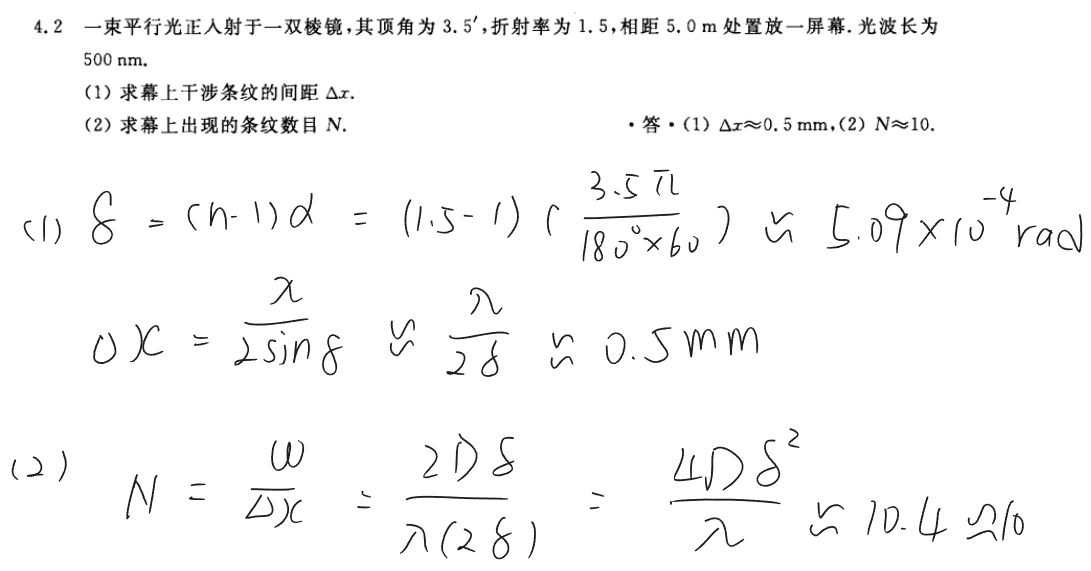
\includegraphics[width=\linewidth, height=0.88\textheight, keepaspectratio]{习题 4.2.png}
\end{figure}
\clearpage

\section*{习题 4.5}
\begin{figure}[H]
  \centering
  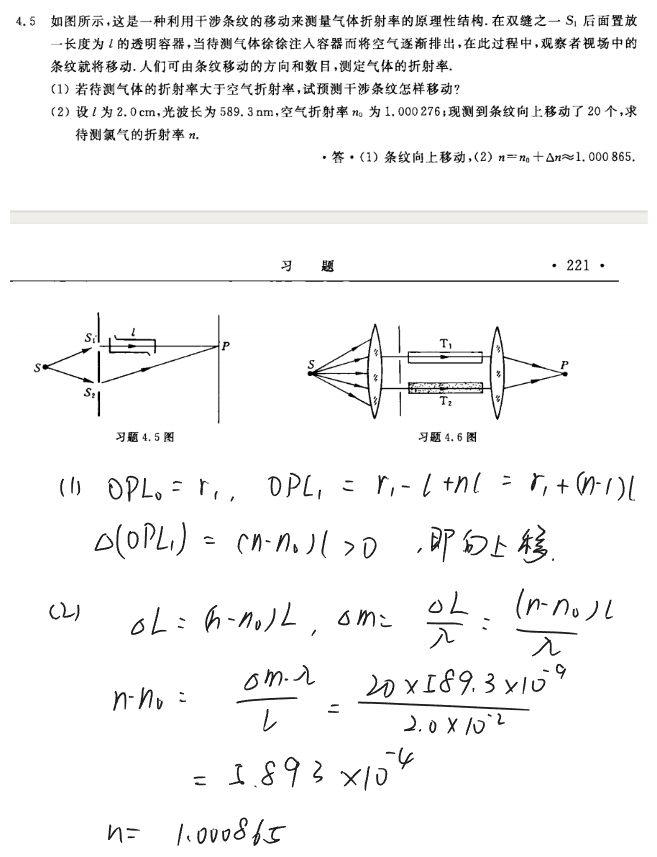
\includegraphics[width=\linewidth, height=0.88\textheight, keepaspectratio]{习题 4.5.png}
\end{figure}
\clearpage

\section*{习题 4.7}
\begin{figure}[H]
  \centering
  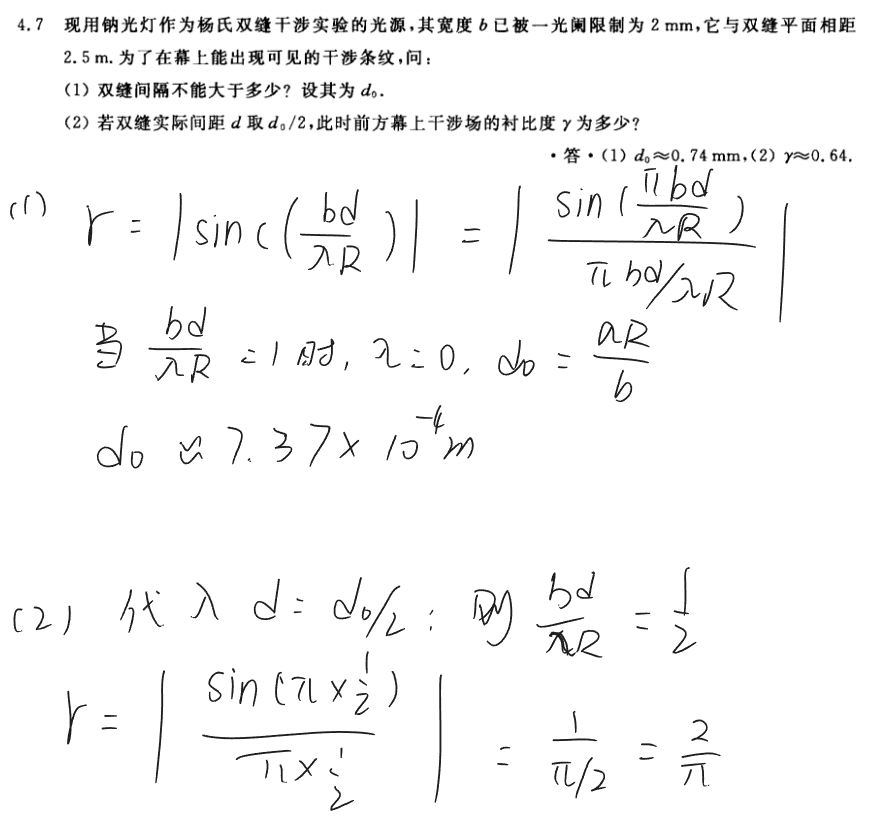
\includegraphics[width=\linewidth, height=0.88\textheight, keepaspectratio]{习题 4.7.png}
\end{figure}
\clearpage

\section*{习题 4.8}
\begin{figure}[H]
  \centering
  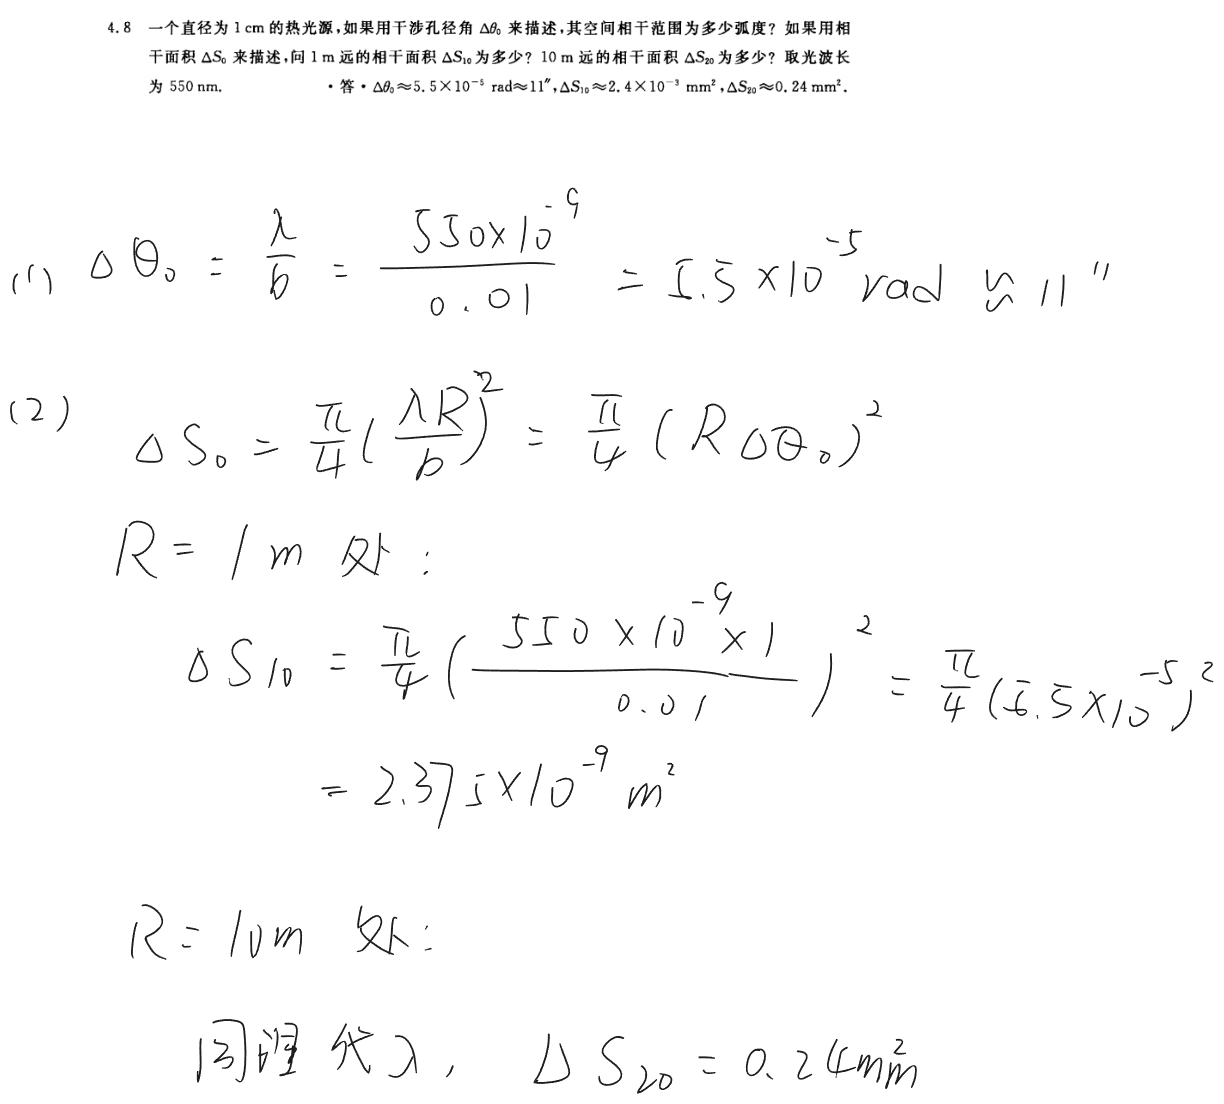
\includegraphics[width=\linewidth, height=0.88\textheight, keepaspectratio]{习题 4.8.png}
\end{figure}
\clearpage

\section*{习题 4.9}
\begin{figure}[H]
  \centering
  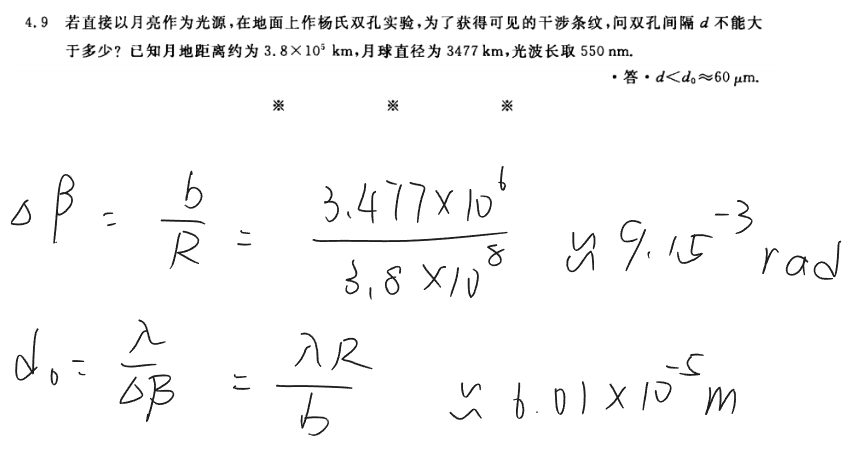
\includegraphics[width=\linewidth, height=0.88\textheight, keepaspectratio]{习题 4.9.png}
\end{figure}
\clearpage

\section*{习题 4.13}
\begin{figure}[H]
  \centering
  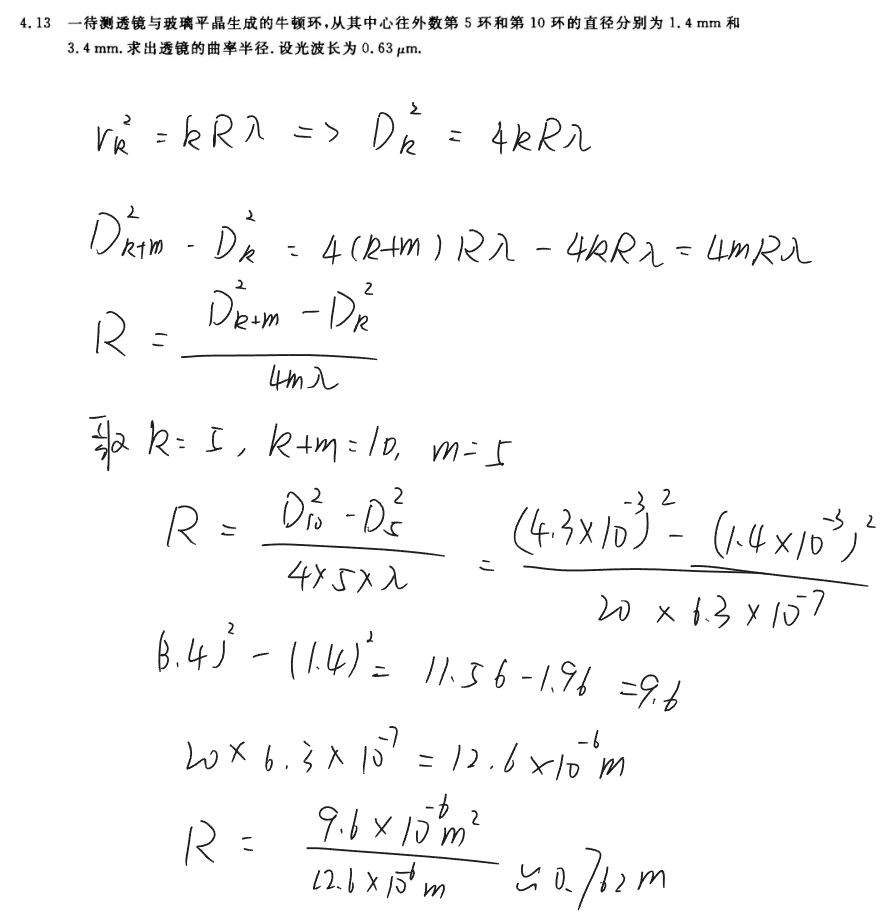
\includegraphics[width=\linewidth, height=0.88\textheight, keepaspectratio]{习题 4.13.png}
\end{figure}
\clearpage

\section*{习题 4.10}
\begin{figure}[H]
  \centering
  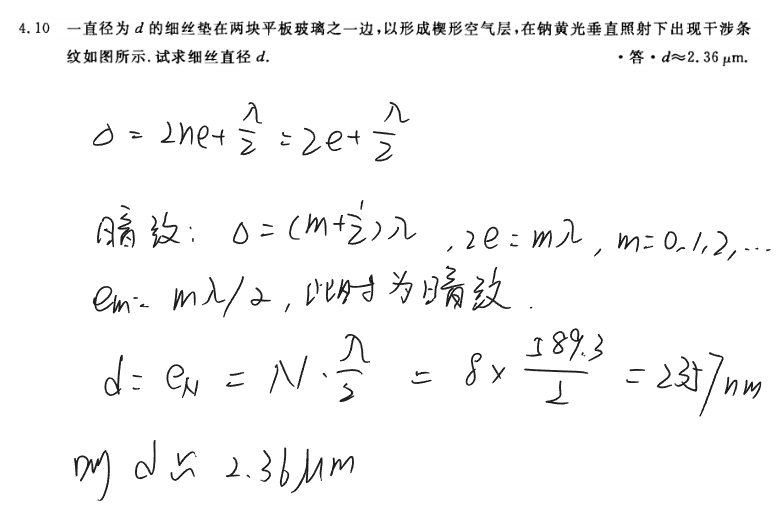
\includegraphics[width=\linewidth, height=0.88\textheight, keepaspectratio]{习题 4.10.png}
\end{figure}
\clearpage

\section*{习题 4.18}
\begin{figure}[H]
  \centering
  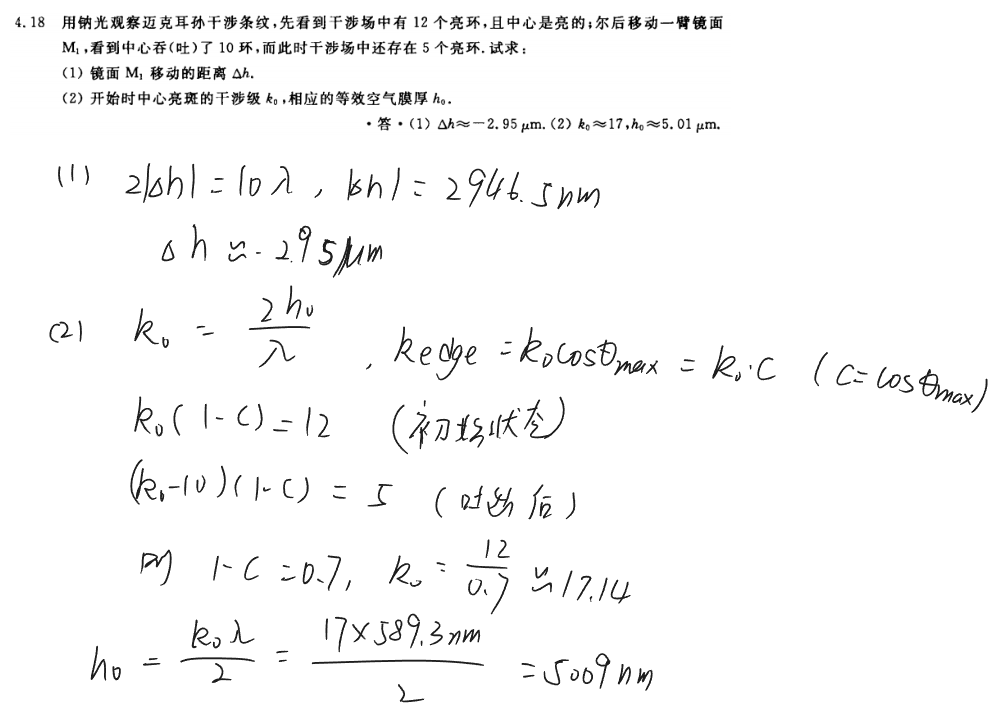
\includegraphics[width=\linewidth, height=0.88\textheight, keepaspectratio]{习题 4.18.png}
\end{figure}
\clearpage

\end{document}
